%=========================================================
% Exam-Oriented Notes
% Modern Computing and Python Programming (26ESCC106)
% Module 1 : Evolution of Computing (Text Book 1: 1.1 - 1.1.2)
% Compile using XeLaTeX:  latexmk -xelatex notes.tex
%=========================================================

\documentclass[11pt,a4paper]{article}

%---------------------------------------------------------
% Packages
%---------------------------------------------------------
\usepackage[margin=2cm,headheight=28pt,headsep=12pt]{geometry}
\usepackage{fontspec}
\setmainfont{Times New Roman}
\usepackage{amsmath,amssymb}
\usepackage{graphicx}
\usepackage{booktabs}
\usepackage{array}
\usepackage{tabularx}
\usepackage{enumitem}
\usepackage{fancyhdr}
\usepackage{xcolor}
\usepackage[most]{tcolorbox}
\usepackage{tikz}
\usetikzlibrary{arrows.meta,positioning,shapes.geometric,shapes.misc,shapes.symbols,fit,calc}
\usepackage[hidelinks]{hyperref}
\usepackage{titlesec}

\setlist{itemsep=2pt,topsep=3pt,leftmargin=*}
\setlength{\parindent}{0pt}
\setlength{\parskip}{5pt}
\setlength{\emergencystretch}{1.5em}

%---------------------------------------------------------
% Header / Footer
%---------------------------------------------------------
\pagestyle{fancy}
\fancyhf{}
\fancyhead[L]{
\includegraphics[height=22pt]{images/MITE_logo.png}}
\fancyhead[C]{\small\textbf{Modern Computing and Python Programming (26ESCC106)}\\ \footnotesize Module 1 Notes: Evolution of Computing}
\fancyhead[R]{\small Manjunath Prasad H. R.}
\fancyfoot[C]{\small Page \thepage}
\renewcommand{\headrulewidth}{0.6pt}

%---------------------------------------------------------
% Headings
%---------------------------------------------------------
\titleformat{\section}{\Large\bfseries}{\thesection.}{0.5em}{}
\titleformat{\subsection}{\large\bfseries}{\thesubsection}{0.5em}{}
\titlespacing*{\section}{0pt}{12pt}{6pt}
\titlespacing*{\subsection}{0pt}{8pt}{4pt}

%---------------------------------------------------------
% Boxes
%---------------------------------------------------------
% Exam question box: \question{marks}{question text}
\newtcolorbox{qbox}{enhanced,colback=black!6,colframe=black,boxrule=0.6pt,arc=1pt,
  left=6pt,right=6pt,top=4pt,bottom=4pt,before skip=6pt,after skip=6pt}
\newcommand{\question}[2]{%
\begin{qbox}\textbf{Q.} #2\unskip\nobreak\hfil\penalty50\hskip2em\hbox{}\nobreak\hfil\textbf{[#1 Marks]}{\parfillskip=0pt\par}\end{qbox}}

\newtcolorbox{defbox}{enhanced,colback=white,colframe=black,boxrule=0.5pt,arc=1pt,
  left=6pt,right=6pt,top=3pt,bottom=3pt,before skip=5pt,after skip=5pt}

\newtcolorbox{keybox}{enhanced,breakable,colback=white,colframe=black,boxrule=0.5pt,arc=1pt,
  left=6pt,right=6pt,top=3pt,bottom=3pt,before skip=6pt,after skip=6pt,
  title={Key Points to Remember},colbacktitle=black!12,coltitle=black,fonttitle=\bfseries}

%---------------------------------------------------------
% TikZ styles (same as the handout)
%---------------------------------------------------------
\tikzset{
  box/.style={draw,rounded corners=2pt,align=center,font=\small,minimum height=0.8cm,inner sep=4pt},
  pc/.style={draw,minimum width=1.1cm,minimum height=0.7cm,font=\scriptsize,align=center},
  arr/.style={-{Stealth[length=2.5mm]},thick},
  darr/.style={{Stealth[length=2.5mm]}-{Stealth[length=2.5mm]},thick},
}

\newcommand{\figcap}[1]{\\[2pt]{\footnotesize\textit{#1}}}

%=========================================================
\begin{document}
%=========================================================

\begin{center}
{\LARGE\bfseries Module 1: Evolution of Computing}\\[4pt]
{\large Exam-Oriented Notes}\\[4pt]
Modern Computing and Python Programming (26ESCC106)\\
Text Book 1: Kai Hwang, Geoffrey C. Fox and Jack J. Dongarra, \textit{Distributed and Cloud Computing: From Parallel Processing to the Internet of Things}, Morgan Kaufmann, 2012 (Sections 1.1, 1.1.1, 1.1.2)\\[6pt]
\textbf{Manjunath Prasad H. R.}, Assistant Professor, Department of AIML, MITE
\end{center}

\begin{tcolorbox}[colback=white,colframe=black,boxrule=0.5pt,arc=1pt,title={Note on Preparation},colbacktitle=black!12,coltitle=black,fonttitle=\bfseries]
\small This document was prepared by \textbf{Manjunath Prasad H. R.}, Course Coordinator, Modern Computing and Python Programming (26ESCC106), and Assistant Professor, Department of AIML, MITE. AI assistance was used to draft and to typeset the document in \LaTeX. However, the answers are handpicked manually and this was prepared under his direction on the source textbook, syllabus scope, template, diagram policy and the 6/8-mark exam format. All content has been reviewed by the course coordinator.
\end{tcolorbox}

\begin{tcolorbox}[colback=black!5,colframe=black,boxrule=0.5pt,arc=1pt,title={How to Use These Notes},colbacktitle=black!12,coltitle=black,fonttitle=\bfseries]
\begin{itemize}
\item Each section begins with a typical university-style question and its marks (6 or 8).
\item The content below the question is written so that it can be reproduced as the answer.
\item \textbf{6-mark answer:} definition + 5--6 explained points (+ a diagram where asked).
\item \textbf{8-mark answer:} introduction + 6--8 explained points + a neat, labelled diagram + a concluding sentence.
\item Diagrams are the same as those in the lecture slides and handout. Always label every box and arrow.
\item A complete question bank with section references is given at the end (Section~\ref{sec:qbank}).
\end{itemize}
\end{tcolorbox}
\clearpage
\tableofcontents
\clearpage

%=========================================================
\section{Scalable Computing over the Internet}
%=========================================================

\question{6}{What is scalable computing over the Internet? Explain how computing has changed from centralized to parallel and distributed computing.}

\begin{defbox}
\textbf{Scalable computing} is computing in which a system can handle a growing amount of work simply by adding more resources such as computers, processors, and storage. \textbf{Scalable computing over the Internet} means using many computers connected through the Internet, instead of one centralized computer, to solve large-scale problems.
\end{defbox}

Over the past 60 years, computing technology has gone through a series of platform and environment changes. Instead of using a single centralized computer to solve computational problems, a parallel and distributed computing system uses \textbf{multiple computers} to solve large-scale problems over the Internet.

\textbf{Evolutionary changes have taken place in four areas:}
\begin{enumerate}
\item \textbf{Machine architecture:} The internal design of computers has changed from single processors to multicore processors, clusters, and massively parallel systems.
\item \textbf{Operating system platform:} Operating systems have evolved from single-machine OSes to systems that manage many networked and virtualized machines.
\item \textbf{Network connectivity:} Computers that once worked alone are now linked by high-speed wired and wireless networks and by the Internet.
\item \textbf{Application workload:} Applications now serve millions of users simultaneously and handle huge volumes of data.
\end{enumerate}

\textbf{Consequences of this change:}
\begin{enumerate}[resume]
\item Computing has become \textbf{data-intensive}, i.e., the main challenge is storing, moving, and processing very large amounts of data.
\item Computing has become \textbf{network-centric}, i.e., the work depends on many computers communicating over a network.
\item Large-scale Internet applications such as web search, online banking, e-mail, and social networking have significantly enhanced the \textbf{quality of life} and information services in society.
\end{enumerate}

\begin{center}
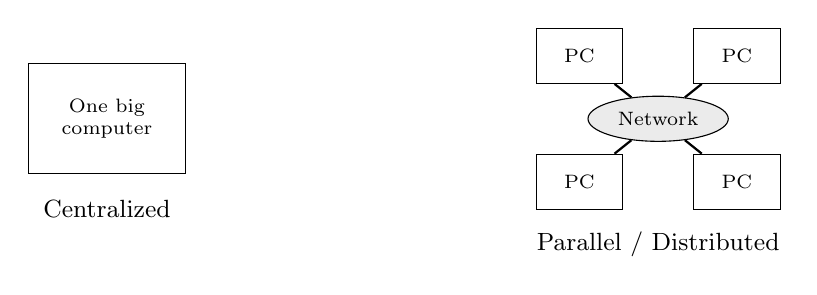
\begin{tikzpicture}[node distance=0.6cm]
\node[pc,minimum width=2cm,minimum height=1.4cm] (c) {One big\\computer};
\node[below=0.2cm of c,font=\small] {Centralized};
\node[pc] (a) at (6,0.8) {PC};
\node[pc] (b) at (8,0.8) {PC};
\node[pc] (d) at (6,-0.8) {PC};
\node[pc] (e) at (8,-0.8) {PC};
\node[draw,ellipse,font=\scriptsize,fill=black!8] (n) at (7,0) {Network};
\foreach \x in {a,b,d,e} \draw[thick] (\x)--(n);
\node[font=\small] at (7,-1.6) {Parallel / Distributed};
\end{tikzpicture}
\figcap{Figure 1: Centralized computing versus parallel/distributed computing}
\end{center}

\textbf{Example:} A single Google search is answered by thousands of servers working together, not by one computer.

\begin{keybox}
\begin{itemize}
\item Centralized $\rightarrow$ parallel and distributed computing over the Internet.
\item Four areas of change: architecture, OS platform, network connectivity, application workload.
\item Result: computing is data-intensive and network-centric.
\end{itemize}
\end{keybox}

%=========================================================
\section{The Age of Internet Computing}
%=========================================================

\question{6}{Explain the age of Internet computing. Why is the Linpack benchmark no longer optimal for measuring system performance?}

Billions of people use the Internet every day. This has changed the requirements placed on computer systems in the following ways:

\begin{enumerate}
\item \textbf{Huge concurrent demand:} Supercomputer sites and large data centers must provide high-performance computing services to huge numbers of Internet users \textbf{concurrently} (at the same time).
\item \textbf{Linpack is no longer optimal:} The \textbf{Linpack Benchmark} measures how fast a computer solves a large system of linear equations (in flops). It is suited to ranking HPC systems by raw speed, but it does not measure how well a system serves millions of simultaneous users. Hence it is no longer the best measure of performance for Internet computing.
\item \textbf{Shift to HTC:} The emergence of computing clouds demands \textbf{High-Throughput Computing (HTC)} systems built with parallel and distributed computing technologies.
\item \textbf{Upgrading data centers:} Data centers must be upgraded with
  \begin{itemize}
  \item fast servers,
  \item large storage systems, and
  \item high-bandwidth networks.
  \end{itemize}
\item \textbf{Purpose:} The aim is to advance network-based computing and web services using emerging technologies.
\end{enumerate}

\begin{center}
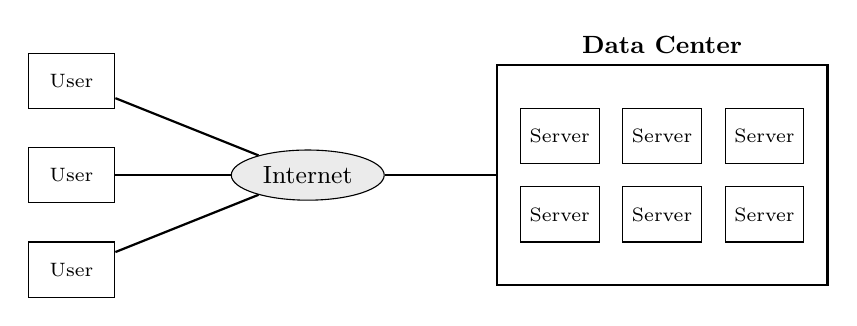
\begin{tikzpicture}
\foreach \i in {0,1,2} \node[pc] (u\i) at (0,1.2-\i*1.2) {User};
\node[draw,ellipse,fill=black!8,font=\small] (net) at (3,0) {Internet};
\node[draw,thick,minimum width=4.2cm,minimum height=2.8cm] (dc) at (7.5,0) {};
\node[font=\small\bfseries,above] at (dc.north) {Data Center};
\foreach \x in {0,1,2} \foreach \y in {0,1} \node[pc,minimum width=0.9cm] at (6.2+\x*1.3,0.5-\y*1) {Server};
\foreach \i in {0,1,2} \draw[thick] (u\i)--(net);
\draw[thick] (net)--(dc.west);
\end{tikzpicture}
\figcap{Figure 2: Many Internet users served concurrently by a data center}
\end{center}

\begin{keybox}
\begin{itemize}
\item Billions of users $\Rightarrow$ concurrent service from data centers.
\item Linpack measures raw speed, not service to many users $\Rightarrow$ not optimal.
\item Clouds demand HTC systems; data centers need fast servers, storage, and high-bandwidth networks.
\end{itemize}
\end{keybox}

%=========================================================
\section{The Platform Evolution: Five Generations of Computers}
%=========================================================

\question{6}{Explain the platform evolution of computer technology through five generations with suitable examples.}

Computer technology has gone through \textbf{five generations} of development. Each generation lasted \textbf{10 to 20 years}, and successive generations \textbf{overlapped by about 10 years}.

\begin{enumerate}
\item \textbf{1950--1970: Mainframes.} A handful of large, expensive mainframes such as the \textbf{IBM 360} and \textbf{CDC 6400} were built to satisfy the demands of large businesses and government organizations.
\item \textbf{1960--1980: Minicomputers.} Lower-cost minicomputers such as the \textbf{DEC PDP 11} and \textbf{VAX Series} became popular among small businesses and on college campuses.
\item \textbf{1970--1990: Personal computers.} Personal computers built with \textbf{VLSI microprocessors} came into widespread use by individuals and offices.
\item \textbf{1980--2000: Portable and pervasive devices.} Massive numbers of portable computers (laptops) and pervasive devices appeared in both \textbf{wired and wireless} applications.
\item \textbf{Since 1990: HPC and HTC systems.} The use of HPC and HTC systems hidden in \textbf{clusters, grids, and Internet clouds} has proliferated. These are used by consumers as well as by high-end web-scale computing and information services.
\end{enumerate}

\begin{center}
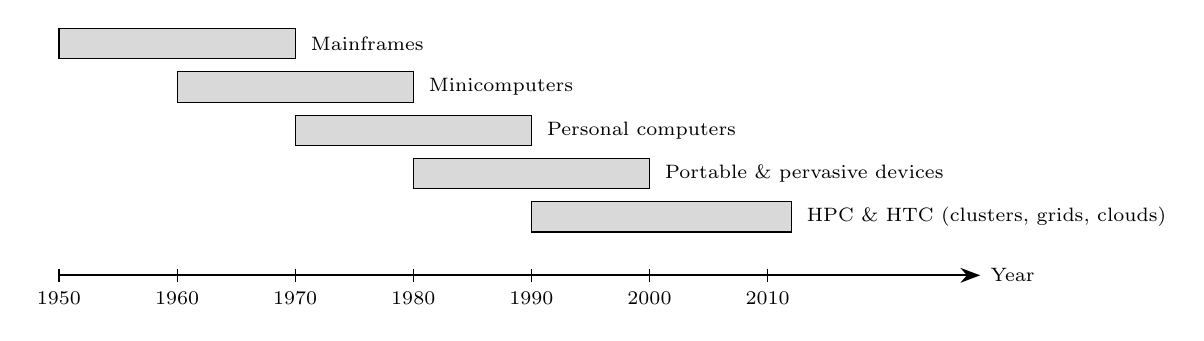
\begin{tikzpicture}[x=0.15cm,y=0.55cm]
\draw[arr] (0,0)--(78,0) node[right,font=\scriptsize]{Year};
\foreach \yr in {1950,1960,1970,1980,1990,2000,2010} {\draw ({\yr-1950},0.15)--({\yr-1950},-0.15) node[below,font=\scriptsize]{\yr};}
\foreach \s/\e/\lab/\r in {0/20/{Mainframes}/5,10/30/{Minicomputers}/4,20/40/{Personal computers}/3,30/50/{Portable \& pervasive devices}/2,40/62/{HPC \& HTC (clusters, grids, clouds)}/1}
{\fill[black!15,draw=black] (\s,\r) rectangle (\e,\r+0.7); \node[right,font=\scriptsize] at (\e+0.5,\r+0.35) {\lab};}
\end{tikzpicture}
\figcap{Figure 3: Overlapping generations of computer platforms}
\end{center}

\begin{center}
\renewcommand{\arraystretch}{1.25}
\small
\begin{tabular}{|p{2cm}|p{3.6cm}|p{4.2cm}|p{3.8cm}|}
\hline
\textbf{Period} & \textbf{Platform} & \textbf{Examples} & \textbf{Main Users} \\ \hline
1950--1970 & Mainframes & IBM 360, CDC 6400 & Large businesses, government \\ \hline
1960--1980 & Minicomputers & DEC PDP 11, VAX Series & Small businesses, colleges \\ \hline
1970--1990 & Personal computers & PCs with VLSI microprocessors & Individuals, offices \\ \hline
1980--2000 & Portable \& pervasive devices & Laptops, wired/wireless devices & Mobile users \\ \hline
Since 1990 & HPC and HTC systems & Clusters, grids, Internet clouds & Consumers, web-scale services \\ \hline
\end{tabular}
\end{center}

\textbf{General trend:} The general computing trend is to leverage \textbf{shared web resources} and \textbf{massive amounts of data} over the Internet.

%=========================================================
\section{Evolutionary Trend toward Parallel, Distributed, and Cloud Computing}
%=========================================================

\question{8}{With a neat diagram, explain the evolutionary trend toward parallel, distributed, and cloud computing.}

Figure 4 (Figure 1.1 of the textbook) illustrates the evolution of HPC and HTC systems and how they lead to grids, clouds, web services, and the Internet of Things.

\begin{center}
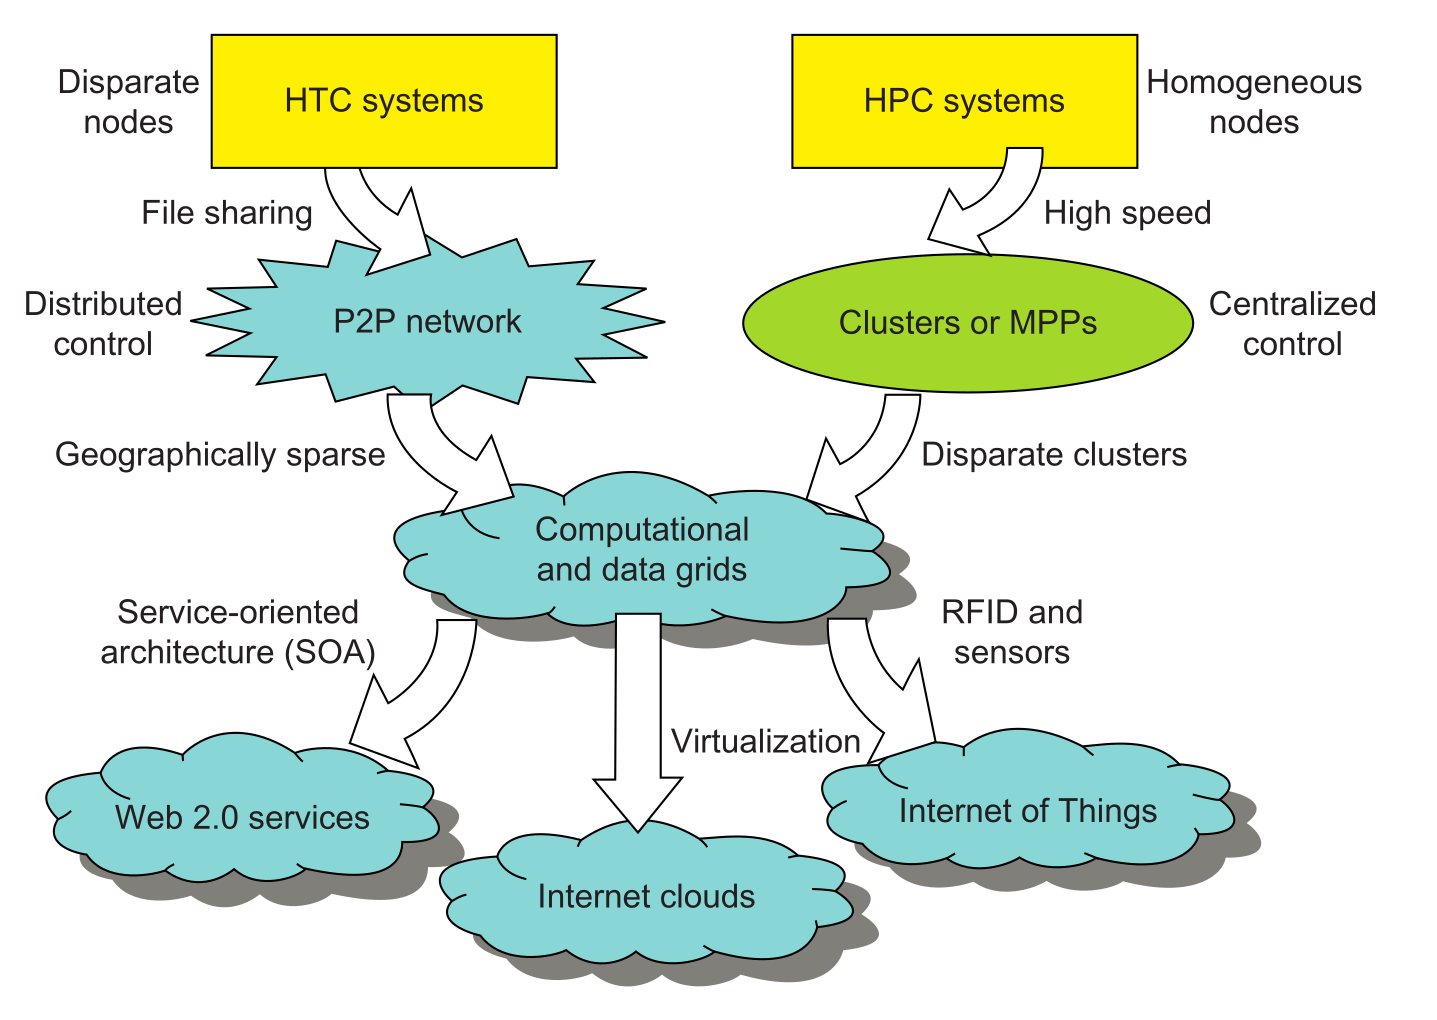
\includegraphics[width=0.62\linewidth]{images/Fig1_1_evolution_trend.png}
\figcap{Figure 4: Evolutionary trend toward parallel, distributed, and cloud computing with clusters, MPPs, P2P networks, grids, clouds, web services, and the Internet of Things (Text Book 1, Fig.\ 1.1)}
\end{center}

\textbf{Explanation of the figure:}
\begin{enumerate}
\item \textbf{Two starting points:} The figure starts with \textbf{HTC systems} (left) and \textbf{HPC systems} (right).
\item \textbf{HPC side:} Supercomputers, also called \textbf{Massively Parallel Processors (MPPs)}, are gradually replaced by \textbf{clusters} of cooperative computers, because organizations want to share computing resources. HPC systems use \textbf{homogeneous nodes}, \textbf{centralized control}, and aim for \textbf{high speed}.
\item \textbf{Cluster:} A cluster is a collection of homogeneous compute nodes that are physically connected in close range to one another.
\item \textbf{HTC side:} \textbf{Peer-to-peer (P2P) networks} are formed for distributed \textbf{file sharing} and \textbf{content delivery}. A P2P system is built over many client machines that are globally distributed. HTC systems use \textbf{disparate nodes} and \textbf{distributed control}.
\item \textbf{Focus of HTC platforms:} P2P, cloud computing, and web service platforms are focused more on HTC applications than on HPC applications.
\item \textbf{Grids:} Clustering technology (\textbf{disparate clusters}) and P2P technology (\textbf{geographically sparse} peers) together lead to \textbf{computational and data grids}.
\item \textbf{From grids to new paradigms:}
  \begin{itemize}
  \item \textbf{Service-oriented architecture (SOA)} leads to \textbf{Web 2.0 services}.
  \item \textbf{Virtualization} leads to \textbf{Internet clouds}.
  \item \textbf{RFID and sensors} lead to the \textbf{Internet of Things}.
  \end{itemize}
\end{enumerate}

\textbf{Labels on the arrows of Figure 1.1:}

\begin{center}
\renewcommand{\arraystretch}{1.3}
\small
\begin{tabular}{|p{3cm}|p{5.4cm}|p{5.4cm}|}
\hline
\textbf{Feature} & \textbf{HPC path (Clusters / MPPs)} & \textbf{HTC path (P2P networks)} \\ \hline
Type of nodes & Homogeneous (same kind of computers) & Disparate (different kinds of computers) \\ \hline
Control & Centralized control & Distributed control \\ \hline
Location & Physically close & Geographically sparse \\ \hline
Purpose & High speed & File sharing \\ \hline
\end{tabular}
\end{center}

The difference between centralized and distributed control and between client--server and P2P organization is shown below.

\begin{center}
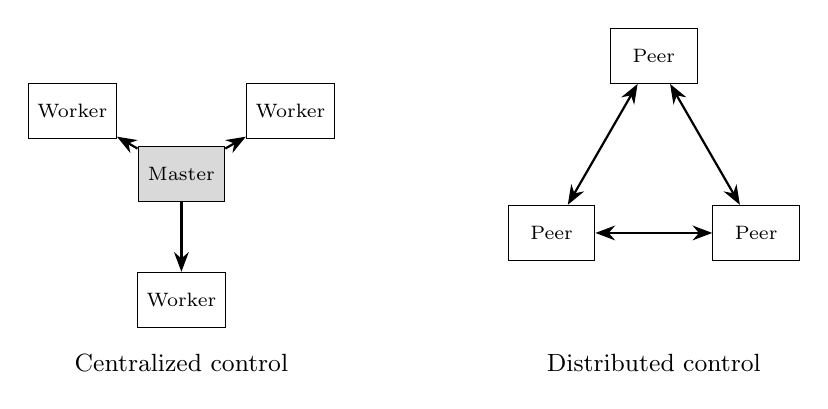
\begin{tikzpicture}
\node[pc,fill=black!15] (m) at (0,0) {Master};
\foreach \a in {30,150,270} \node[pc] (w\a) at ($(m)+(\a:1.6)$) {Worker};
\foreach \a in {30,150,270} \draw[arr] (m)--(w\a);
\node[font=\small] at (0,-2.4) {Centralized control};
\foreach \a in {90,210,330} \node[pc] (q\a) at ($(6,0)+(\a:1.5)$) {Peer};
\draw[darr] (q90)--(q210); \draw[darr] (q210)--(q330); \draw[darr] (q330)--(q90);
\node[font=\small] at (6,-2.4) {Distributed control};
\end{tikzpicture}
\figcap{Figure 5: Centralized control (HPC side) versus distributed control (HTC side)}
\end{center}

\begin{center}
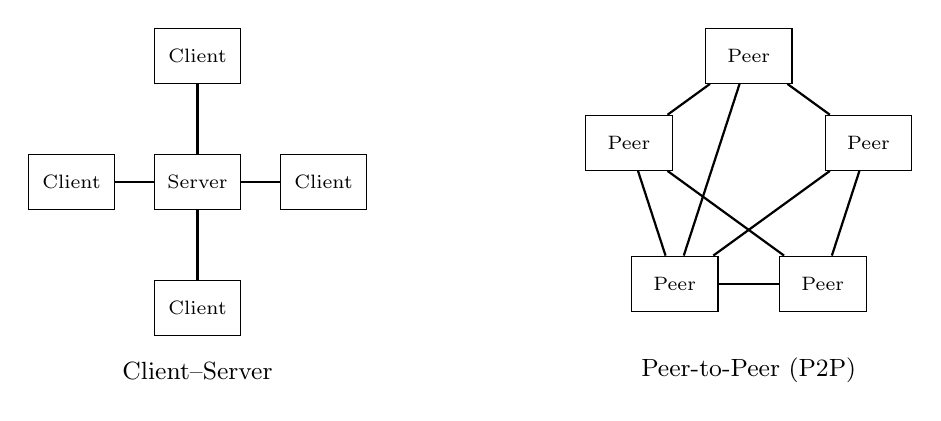
\begin{tikzpicture}
\node[pc] (s) at (0,0) {Server};
\foreach \a in {0,90,180,270} \node[pc] (c\a) at ($(s)+(\a:1.6)$) {Client};
\foreach \a in {0,90,180,270} \draw[thick] (s)--(c\a);
\node[font=\small] at (0,-2.4) {Client--Server};
\foreach \a in {90,162,234,306,18} \node[pc] (p\a) at ($(7,0)+(\a:1.6)$) {Peer};
\foreach \a/\b in {90/162,162/234,234/306,306/18,18/90,90/234,162/306,234/18} \draw[thick] (p\a)--(p\b);
\node[font=\small] at (7,-2.4) {Peer-to-Peer (P2P)};
\end{tikzpicture}
\figcap{Figure 6: Client--server versus peer-to-peer organization}
\end{center}

\textbf{Conclusion:} Both HPC and HTC paths converge into grids, and grids in turn give rise to Web 2.0 services, Internet clouds, and the IoT.

%=========================================================
\section{High-Performance Computing and High-Throughput Computing}
%=========================================================

\subsection{High-Performance Computing (HPC)}

\question{6}{What is High-Performance Computing (HPC)? Explain its characteristics.}

\begin{defbox}
\textbf{High-Performance Computing (HPC)} is the use of supercomputers and clusters to solve large and complex problems as \textbf{fast as possible}. HPC systems emphasize \textbf{raw speed performance}.
\end{defbox}

\begin{enumerate}
\item \textbf{Focus on speed:} For many years, HPC systems have emphasized raw speed performance, i.e., how fast a single large problem can be solved.
\item \textbf{Growth in speed:} The speed of HPC systems increased from \textbf{Gflops} ($10^{9}$ floating-point operations per second) in the early 1990s to \textbf{Pflops} ($10^{15}$ flops) in 2010.
\item \textbf{Driving force:} This improvement was driven mainly by the demands of the \textbf{scientific, engineering, and manufacturing} communities.
\item \textbf{Measurement:} The \textbf{Top 500} most powerful computer systems in the world are ranked by their floating-point speed in \textbf{Linpack benchmark} results.
\item \textbf{Limited users:} The number of supercomputer users is limited to \textbf{less than 10\%} of all computer users.
\item \textbf{Majority of users:} Today, most users use desktop computers or large servers for Internet searches and market-driven computing tasks, not supercomputers.
\end{enumerate}

\textbf{Examples:} Weather forecasting, earthquake simulation, and genome analysis.

\subsection{High-Throughput Computing (HTC)}

\question{6}{What is High-Throughput Computing (HTC)? Why is market-oriented computing shifting from HPC to HTC?}

\begin{defbox}
\textbf{High-Throughput Computing (HTC)} is computing that emphasizes \textbf{high-flux computing}, i.e., completing the \textbf{largest number of tasks per unit of time}, rather than finishing one task as fast as possible.
\end{defbox}

\begin{enumerate}
\item \textbf{Strategic change:} The development of market-oriented high-end computing systems is undergoing a strategic change from an \textbf{HPC paradigm} to an \textbf{HTC paradigm}.
\item \textbf{High-flux computing:} The HTC paradigm pays more attention to high-flux computing, i.e., a very high flow of tasks through the system.
\item \textbf{Main applications:} Internet searches and web services used by \textbf{millions of users simultaneously}.
\item \textbf{Performance goal:} The performance goal shifts to \textbf{throughput}, i.e., the number of tasks completed per unit of time.
\item \textbf{Beyond speed:} HTC must improve batch processing speed and must also address the acute problems of
  \begin{itemize}
  \item cost,
  \item energy savings,
  \item security, and
  \item reliability
  \end{itemize}
  at data and enterprise computing centers.
\end{enumerate}

\textbf{Example:} Millions of students checking their examination results on a university website at the same time.

\subsection{HPC versus HTC}

\question{8}{Differentiate between HPC and HTC systems with a neat diagram and suitable examples.}

\begin{center}
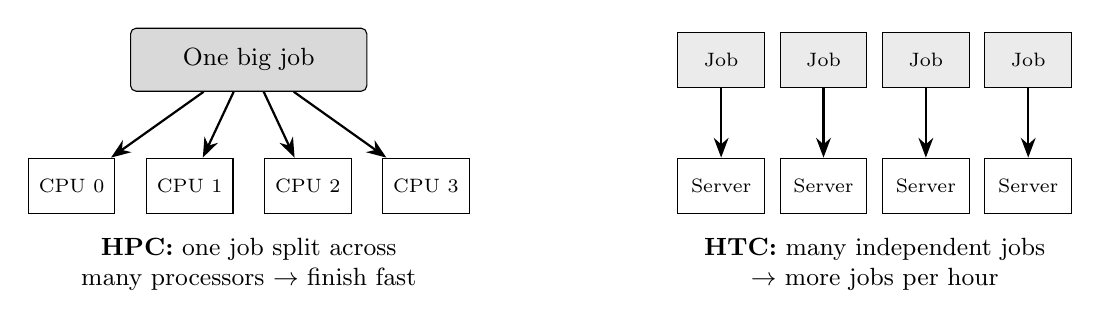
\begin{tikzpicture}
\node[box,minimum width=3cm,fill=black!15] (j) at (0,0) {One big job};
\foreach \i in {0,1,2,3} \node[pc] (p\i) at (-2.25+\i*1.5,-1.6) {CPU \i};
\foreach \i in {0,1,2,3} \draw[arr] (j)--(p\i);
\node[font=\small,align=center] at (0,-2.6) {\textbf{HPC:} one job split across\\many processors $\rightarrow$ finish fast};
\foreach \i in {0,1,2,3} {\node[pc,fill=black!8] (t\i) at (6+\i*1.3,0) {Job}; \node[pc] (s\i) at (6+\i*1.3,-1.6) {Server}; \draw[arr] (t\i)--(s\i);}
\node[font=\small,align=center] at (7.95,-2.6) {\textbf{HTC:} many independent jobs\\$\rightarrow$ more jobs per hour};
\end{tikzpicture}
\figcap{Figure 7: HPC versus HTC}
\end{center}

\begin{center}
\renewcommand{\arraystretch}{1.35}
\small
\begin{tabular}{|c|p{3cm}|p{5.2cm}|p{5.2cm}|}
\hline
\textbf{Sl.} & \textbf{Aspect} & \textbf{High-Performance Computing} & \textbf{High-Throughput Computing} \\ \hline
1 & Goal & Solve one big problem as fast as possible & Complete as many tasks as possible per unit time \\ \hline
2 & Emphasis & Raw speed performance & High-flux computing \\ \hline
3 & Measure & Speed in flops (Linpack benchmark, Top 500) & Throughput (tasks completed per unit time) \\ \hline
4 & Typical systems & Supercomputers, MPPs, clusters & P2P networks, clouds, web service platforms \\ \hline
5 & Users & Scientists and engineers ($<$10\% of users) & General Internet users (millions) \\ \hline
6 & Driven by & Scientific, engineering, and manufacturing communities & Market-oriented, business computing \\ \hline
7 & Other concerns & Mainly speed & Cost, energy saving, security, reliability \\ \hline
8 & Examples & Weather forecasting, simulations & Web search, e-commerce, social networks \\ \hline
\end{tabular}
\end{center}

\textbf{Analogy:} HPC is like a racing car that carries one passenger very fast; HTC is like a metro train that carries thousands of passengers per hour.

%=========================================================
\section{Three New Computing Paradigms}
%=========================================================

\question{8}{Explain the three new computing paradigms. How has the meaning of the term ``computer'' changed over the years?}

As shown in Figure 1.1, three new technologies have given rise to three new computing paradigms.

\textbf{1. SOA $\rightarrow$ Web 2.0 services}

With the introduction of \textbf{Service-Oriented Architecture (SOA)}, \textbf{Web 2.0 services} became available. In SOA, software is built as a collection of independent services, each doing one job, that communicate over a network using standard interfaces. A service provider publishes its service in a registry, and a service consumer finds and uses it.

\begin{center}
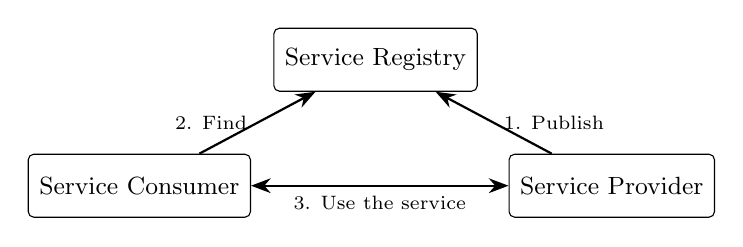
\begin{tikzpicture}
\node[box] (r) at (3,1.6) {Service Registry};
\node[box] (p) at (6,0) {Service Provider};
\node[box] (c) at (0,0) {Service Consumer};
\draw[arr] (p)--node[right,font=\scriptsize]{1. Publish} (r);
\draw[arr] (c)--node[left,font=\scriptsize]{2. Find} (r);
\draw[darr] (c)--node[below,font=\scriptsize]{3. Use the service} (p);
\end{tikzpicture}
\figcap{Figure 8: Service-Oriented Architecture (SOA)}
\end{center}

\textbf{2. Virtualization $\rightarrow$ Internet clouds}

Advances in \textbf{virtualization} made it possible to see the growth of \textbf{Internet clouds} as a new computing paradigm. Virtualization creates several virtual machines (VMs) on one physical computer using a \textbf{hypervisor}; each VM behaves like a separate computer with its own operating system.

\begin{center}
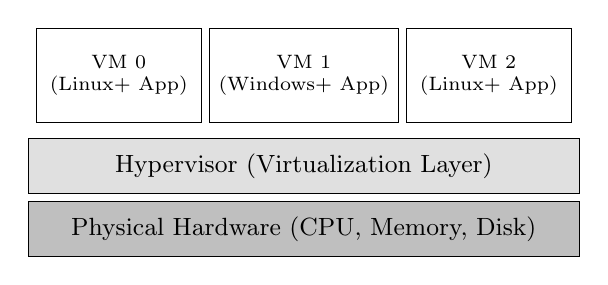
\begin{tikzpicture}
\node[draw,minimum width=7cm,minimum height=0.7cm,fill=black!25,font=\small] (hw) at (0,0) {Physical Hardware (CPU, Memory, Disk)};
\node[draw,minimum width=7cm,minimum height=0.7cm,fill=black!12,font=\small] (hv) at (0,0.8) {Hypervisor (Virtualization Layer)};
\foreach \i/\os in {0/Linux,1/Windows,2/Linux} {\node[draw,minimum width=2.1cm,minimum height=1.2cm,font=\scriptsize,align=center] at (-2.35+\i*2.35,1.95) {VM \i\\(\os + App)};}
\end{tikzpicture}
\figcap{Figure 9: Virtualization --- several virtual machines on one physical machine}
\end{center}

\textbf{3. RFID, GPS, and sensors $\rightarrow$ Internet of Things}

The maturity of \textbf{Radio-Frequency Identification (RFID)}, the \textbf{Global Positioning System (GPS)}, and \textbf{sensor} technologies has triggered the development of the \textbf{Internet of Things (IoT)}.

\begin{center}
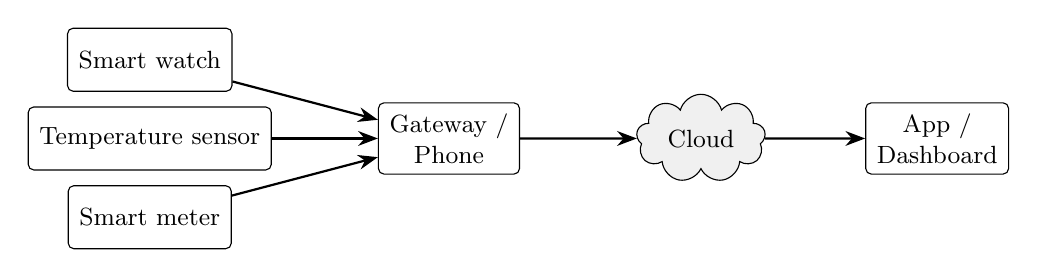
\begin{tikzpicture}
\node[box] (s1) at (0,1) {Smart watch};
\node[box] (s2) at (0,0) {Temperature sensor};
\node[box] (s3) at (0,-1) {Smart meter};
\node[box] (g) at (3.8,0) {Gateway /\\Phone};
\node[draw,cloud,cloud puffs=9,aspect=2,fill=black!6,font=\small] (c) at (7,0) {Cloud};
\node[box] (a) at (10,0) {App /\\Dashboard};
\foreach \i in {1,2,3} \draw[arr] (s\i)--(g);
\draw[arr] (g)--(c); \draw[arr] (c)--(a);
\end{tikzpicture}
\figcap{Figure 10: Internet of Things --- everyday objects connected through the cloud}
\end{center}

\textbf{How the idea of a ``computer'' has changed:}
\begin{enumerate}
\item \textbf{1969 --- Leonard Kleinrock (UCLA):} When the Internet was introduced, he predicted that computer networks would grow into \textbf{computer utilities} that, like electric and telephone utilities, would serve individual homes and offices.
\item \textbf{1984 --- John Gage (Sun Microsystems):} ``\textbf{The network is the computer.}''
\item \textbf{2008 --- David Patterson (UC Berkeley):} ``\textbf{The data center is the computer.}'' He noted the dramatic difference between developing software for millions to use as a service and distributing software to run on PCs.
\item \textbf{Recently --- Rajkumar Buyya (University of Melbourne):} ``\textbf{The cloud is the computer.}''
\end{enumerate}

\textbf{Blurring of paradigms:} The differences among clusters, grids, P2P systems, and clouds may blur in the future. Some view clouds as grids or clusters with modest changes through virtualization; others feel the changes could be major, since clouds are expected to process huge data sets generated by the Internet, social networks, and the IoT.

%=========================================================
\section{Computing Paradigm Distinctions}
%=========================================================

\question{8}{Distinguish between centralized, parallel, distributed, and cloud computing with neat diagrams.}

In general, \textbf{distributed computing is the opposite of centralized computing}. Parallel computing overlaps with distributed computing to a great extent, and cloud computing overlaps with distributed, centralized, and parallel computing.

\textbf{1. Centralized computing}
\begin{itemize}
\item All computer resources are centralized in \textbf{one physical system}.
\item All resources (processors, memory, and storage) are \textbf{fully shared} and \textbf{tightly coupled} within \textbf{one integrated OS}.
\item Many data centers and supercomputers are centralized systems, but they are used in parallel, distributed, and cloud computing applications.
\end{itemize}

\textbf{2. Parallel computing}
\begin{itemize}
\item All processors are either \textbf{tightly coupled} with \textbf{centralized shared memory} or \textbf{loosely coupled} with \textbf{distributed memory}.
\item Some authors refer to this discipline as \textbf{parallel processing}.
\item Interprocessor communication is accomplished through \textbf{shared memory} or via \textbf{message passing}.
\item A system capable of parallel computing is a \textbf{parallel computer}; programs running on it are \textbf{parallel programs}; writing them is \textbf{parallel programming}.
\end{itemize}

\begin{center}
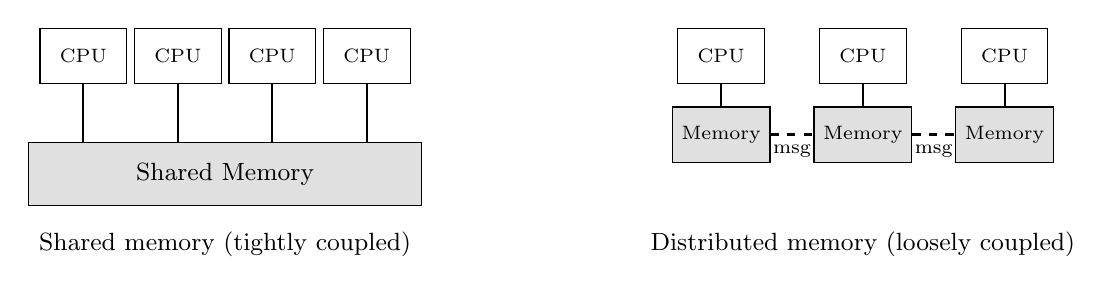
\begin{tikzpicture}
\node[draw,minimum width=5cm,minimum height=0.8cm,fill=black!12,font=\small] (sm) at (0,0) {Shared Memory};
\foreach \i in {0,1,2,3} {\node[pc] (c\i) at (-1.8+\i*1.2,1.5) {CPU}; \draw[thick] (c\i)--(c\i|-sm.north);}
\node[font=\small] at (0,-0.9) {Shared memory (tightly coupled)};
\foreach \i in {0,1,2} {\node[pc] (d\i) at (6.3+\i*1.8,1.5) {CPU}; \node[pc,fill=black!12] (m\i) at (6.3+\i*1.8,0.5) {Memory}; \draw[thick] (d\i)--(m\i);}
\draw[thick,dashed] (m0)--(m1) node[midway,below,font=\scriptsize]{msg}; \draw[thick,dashed] (m1)--(m2) node[midway,below,font=\scriptsize]{msg};
\node[font=\small] at (8.1,-0.9) {Distributed memory (loosely coupled)};
\end{tikzpicture}
\figcap{Figure 11: Parallel computing with shared memory and with distributed memory}
\end{center}

\textbf{3. Distributed computing}
\begin{itemize}
\item It is the field of computer science and engineering that studies \textbf{distributed systems}.
\item A distributed system consists of \textbf{multiple autonomous computers}, each having its \textbf{own private memory}, communicating through a computer network.
\item Information exchange is accomplished through \textbf{message passing}.
\item A program running in a distributed system is a \textbf{distributed program}; writing it is \textbf{distributed programming}.
\end{itemize}

\textbf{4. Cloud computing}
\begin{itemize}
\item An Internet cloud of resources can be either a \textbf{centralized} or a \textbf{distributed} computing system.
\item The cloud applies \textbf{parallel or distributed computing, or both}.
\item Clouds can be built with \textbf{physical or virtualized resources} over large data centers that are centralized or distributed.
\item Some authors consider cloud computing to be a form of \textbf{utility computing} or \textbf{service computing}.
\end{itemize}

\begin{center}
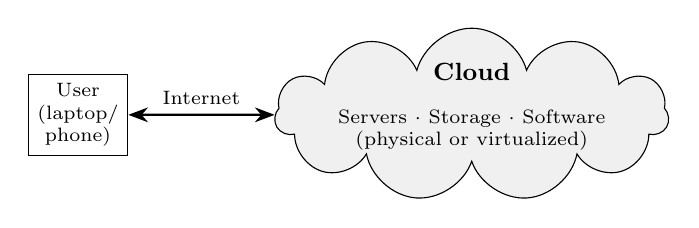
\begin{tikzpicture}
\node[pc] (u) at (0,0) {User\\(laptop/\\phone)};
\node[draw,cloud,cloud puffs=11,aspect=2.2,minimum width=5cm,minimum height=2.2cm,fill=black!6] (cl) at (5,0) {};
\node[font=\small\bfseries] at (5,0.55) {Cloud};
\node[font=\scriptsize,align=center] at (5,-0.2) {Servers $\cdot$ Storage $\cdot$ Software\\(physical or virtualized)};
\draw[darr] (u)--node[above,font=\scriptsize]{Internet} (cl.west);
\end{tikzpicture}
\figcap{Figure 12: Cloud computing}
\end{center}

\begin{center}
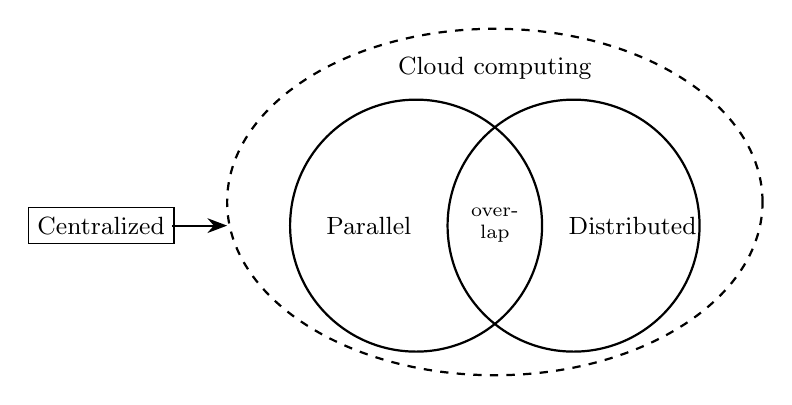
\begin{tikzpicture}
\draw[thick] (0,0) circle (1.6); \node[font=\small] at (-0.6,0) {Parallel};
\draw[thick] (2,0) circle (1.6); \node[font=\small] at (2.75,0) {Distributed};
\node[font=\scriptsize,align=center] at (1,0) {over-\\lap};
\draw[thick,dashed] (1,0.3) ellipse (3.4 and 2.2);
\node[font=\small] at (1,2.0) {Cloud computing};
\node[draw,font=\small] at (-4,0) {Centralized};
\draw[arr] (-3.1,0)--(-2.4,0);
\end{tikzpicture}
\figcap{Figure 13: Overlap of the computing paradigms}
\end{center}

\textbf{Comparison at a glance:}

\begin{center}
\renewcommand{\arraystretch}{1.3}
\small
\begin{tabular}{|p{2.3cm}|p{3.2cm}|p{3.4cm}|p{4.8cm}|}
\hline
\textbf{Paradigm} & \textbf{Memory} & \textbf{Communication} & \textbf{Everyday Analogy} \\ \hline
Centralized & One system, fully shared & Within one OS & One chef cooking in one kitchen \\ \hline
Parallel & Shared or distributed & Shared memory / message passing & Many chefs in one kitchen cooking one meal \\ \hline
Distributed & Private memory per computer & Message passing over a network & Branches of a restaurant chain coordinating by phone \\ \hline
Cloud & Centralized or distributed & Over the Internet & Ordering food online without seeing the kitchen \\ \hline
\end{tabular}
\end{center}

\subsection{Related Terms}

\question{6}{Write short notes on: (a) Concurrent computing (b) Ubiquitous computing (c) Internet of Things (d) Internet computing.}

\begin{enumerate}[label=(\alph*)]
\item \textbf{Concurrent computing / concurrent programming:} An alternative term preferred by some in the high-tech community. It typically refers to the \textbf{union of parallel computing and distributed computing}.
\item \textbf{Ubiquitous computing:} Computing with \textbf{pervasive devices} at \textbf{any place and any time} using wired or wireless communication. Example: smartphones and smart watches used everywhere.
\item \textbf{Internet of Things (IoT):} A networked connection of \textbf{everyday objects}, including computers, sensors, and humans. The IoT is supported by \textbf{Internet clouds} to achieve ubiquitous computing with any object at any place and time (see Figure 10).
\item \textbf{Internet computing:} The broadest term; it covers \textbf{all computing paradigms over the Internet}.
\end{enumerate}

%=========================================================
\section{Distributed System Families and Design Objectives}
%=========================================================

\question{8}{Explain distributed system families. What are the design objectives of future HPC and HTC systems?}

\textbf{Distributed system families:}
\begin{enumerate}
\item \textbf{Grids:} Since the mid-1990s, technologies for building P2P networks and networks of clusters have been consolidated into many national projects that establish \textbf{wide area computing infrastructures}, known as \textbf{computational grids} or \textbf{data grids}.
\item \textbf{Internet clouds:} There is a surge of interest in using Internet cloud resources for \textbf{data-intensive applications}. Clouds result from moving desktop computing to \textbf{service-oriented computing} using server clusters and huge databases at data centers.
\item \textbf{Resource sharing:} Grids and clouds are disparity systems that place great emphasis on \textbf{resource sharing} in hardware, software, and data sets.
\item \textbf{Massively distributed systems:} These systems exploit a high \textbf{degree of parallelism or concurrency} among many machines.
\end{enumerate}

\begin{center}
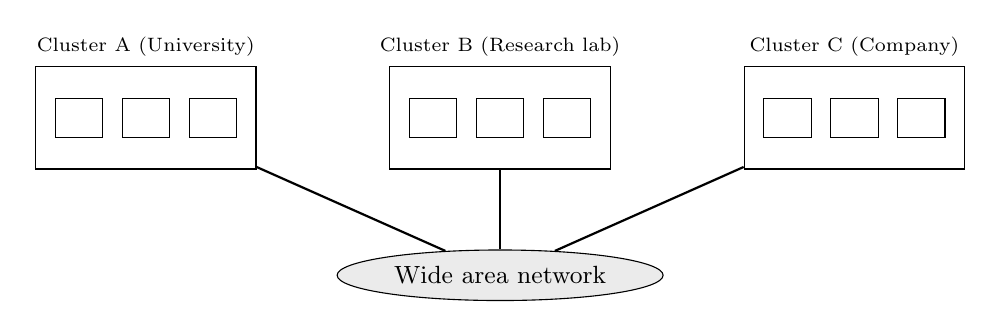
\begin{tikzpicture}
\foreach \i/\lab/\x in {0/{Cluster A (University)}/0,1/{Cluster B (Research lab)}/4.5,2/{Cluster C (Company)}/9} {
  \node[draw,minimum width=2.8cm,minimum height=1.3cm] (k\i) at (\x,0) {};
  \node[font=\scriptsize,above] at (k\i.north) {\lab};
  \foreach \j in {0,1,2} \node[pc,minimum width=0.6cm,minimum height=0.5cm] at (\x-0.85+\j*0.85,0) {};
}
\node[draw,ellipse,fill=black!8,font=\small] (w) at (4.5,-2) {Wide area network};
\foreach \i in {0,1,2} \draw[thick] (k\i)--(w);
\end{tikzpicture}
\figcap{Figure 14: A grid joins clusters owned by different organizations over a wide area network}
\end{center}

\textbf{Scale of these systems (as given in the textbook):}
\begin{itemize}
\item In October 2010, the highest-performing cluster machine, \textbf{Tianhe-1A} (China), had \textbf{86,016 CPU cores} and \textbf{3,211,264 GPU cores}.
\item The largest computational grid connects up to \textbf{hundreds of server clusters}.
\item A typical P2P network may involve \textbf{millions of client machines} working simultaneously.
\item Experimental cloud computing clusters have been built with \textbf{thousands of processing nodes}.
\end{itemize}

\textbf{Need for new design:} Future HPC and HTC systems will demand \textbf{multicore or many-core processors} that handle large numbers of computing threads per core. They must satisfy huge demand in terms of \textbf{throughput, efficiency, scalability, and reliability}. System efficiency is decided by \textbf{speed, programming, and energy} factors (i.e., \textbf{throughput per watt} of energy consumed).

\textbf{Design objectives:}
\begin{enumerate}
\item \textbf{Efficiency:} Measures the utilization rate of resources in an execution model by exploiting massive parallelism in HPC. For HTC, efficiency is related to job throughput, data access, storage, and power efficiency.
\item \textbf{Dependability:} Measures reliability and self-management from the chip to the system and application levels. The purpose is to provide high-throughput service with \textbf{Quality of Service (QoS)} assurance, even under failure conditions.
\item \textbf{Adaptation in the programming model:} Measures the ability to support \textbf{billions of job requests} over massive data sets and virtualized cloud resources under various workload and service models.
\item \textbf{Flexibility in application deployment:} Measures the ability of distributed systems to run well in both \textbf{HPC} (science and engineering) and \textbf{HTC} (business) applications.
\end{enumerate}

%=========================================================
\section{Scalable Computing Trends}
%=========================================================

\question{6}{Explain the scalable computing trends. State Moore's law and Gilder's law.}

Several predictable trends in technology drive computing applications. Designers and programmers want to predict the technological capabilities of future systems.

\begin{enumerate}
\item \textbf{Rules of thumb:} Jim Gray's paper ``\textit{Rules of Thumb in Data Engineering}'' is an excellent example of how technology affects applications and vice versa.
\item \textbf{Moore's law:} Processor speed \textbf{doubles every 18 months}. Moore's law has been valid over the last 30 years, but it is difficult to say whether it will continue to be true in the future.
\item \textbf{Gilder's law:} Network bandwidth has \textbf{doubled each year} in the past.
\item \textbf{Commodity hardware:} The tremendous \textbf{price/performance ratio} of commodity hardware was driven by the desktop, notebook, and tablet computing markets.
\item \textbf{Use in large-scale computing:} This has also driven the adoption of commodity technologies in large-scale computing (clusters and data centers built from ordinary components).
\item \textbf{Distributed systems:} Distributed systems emphasize both \textbf{resource distribution} and \textbf{concurrency}, i.e., a high \textbf{Degree of Parallelism (DoP)}.
\end{enumerate}

\begin{center}
\begin{tikzpicture}[x=0.6cm,y=0.07cm]
\draw[arr] (0,0)--(10.5,0) node[right,font=\scriptsize]{Years};
\draw[arr] (0,0)--(0,72) node[above,font=\scriptsize]{Relative speed};
\draw[very thick,domain=0:9,samples=60] plot (\x,{2^(\x/1.5)});
\foreach \t/\v in {0/1,1.5/2,3/4,4.5/8,6/16,7.5/32,9/64} {\fill (\t,{\v}) circle (1.5pt); \node[left,font=\tiny] at (\t,{\v+2}) {$\times$\v};}
\foreach \t in {0,3,6,9} \node[below,font=\scriptsize] at (\t,0) {\t};
\end{tikzpicture}
\figcap{Figure 15: Moore's law --- doubling every 1.5 years gives 64 times the speed in 9 years}
\end{center}

%=========================================================
\section{Degrees of Parallelism}
%=========================================================

\question{8}{Explain the different degrees of parallelism with neat diagrams.}

\begin{defbox}
The \textbf{Degree of Parallelism (DoP)} is the number of operations or tasks that can be executed at the same time. Parallelism has evolved from fine-grain (bits, instructions) to coarse-grain (tasks, jobs).
\end{defbox}

\textbf{1. Bit-Level Parallelism (BLP)}
\begin{itemize}
\item Fifty years ago, when hardware was bulky and expensive, most computers were designed in a \textbf{bit-serial} fashion.
\item BLP gradually converts bit-serial processing to \textbf{word-level} processing.
\item Users graduated from 4-bit microprocessors to 8-, 16-, 32-, and 64-bit CPUs.
\end{itemize}

\textbf{2. Instruction-Level Parallelism (ILP)}
\begin{itemize}
\item The processor executes \textbf{multiple instructions simultaneously} rather than one at a time.
\item ILP is practised through \textbf{pipelining}, \textbf{superscalar} computing, \textbf{VLIW} (very long instruction word) architectures, and \textbf{multithreading}.
\item ILP requires \textbf{branch prediction}, \textbf{dynamic scheduling}, \textbf{speculation}, and \textbf{compiler support} to work efficiently.
\end{itemize}

\begin{center}
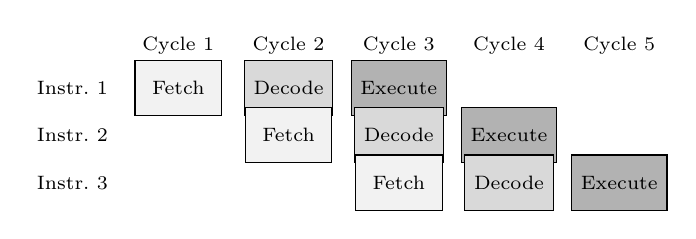
\begin{tikzpicture}[x=1.4cm,y=0.6cm]
\foreach \c in {1,...,5} \node[font=\scriptsize] at (\c,0.9) {Cycle \c};
\foreach \i/\s in {1/1,2/2,3/3} {
  \node[font=\scriptsize,anchor=east] at (0.45,-\i+1) {Instr.\ \i};
  \node[pc,fill=black!5] at (\s,-\i+1) {Fetch};
  \node[pc,fill=black!15] at (\s+1,-\i+1) {Decode};
  \node[pc,fill=black!30] at (\s+2,-\i+1) {Execute};}
\end{tikzpicture}
\figcap{Figure 16: Pipelining (ILP) --- in cycle 3, three instructions are processed at once}
\end{center}

\textbf{3. Data-Level Parallelism (DLP)}
\begin{itemize}
\item One instruction operates on \textbf{many data items} at the same time.
\item DLP was made popular through \textbf{SIMD} (single instruction, multiple data) and \textbf{vector machines} using vector or array instructions.
\item DLP requires even more hardware support and compiler assistance to work properly.
\end{itemize}

\begin{center}
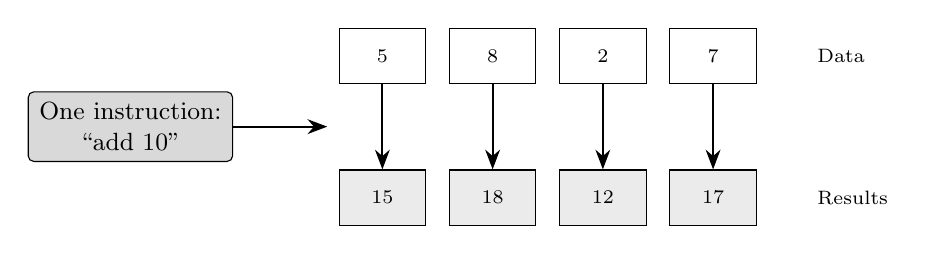
\begin{tikzpicture}
\node[box,fill=black!15] (ins) at (0,0) {One instruction:\\ ``add 10''};
\foreach \i/\d in {0/5,1/8,2/2,3/7} {\node[pc] (d\i) at (3.2+\i*1.4,0.9) {\d}; \node[pc,fill=black!8] (r\i) at (3.2+\i*1.4,-0.9) {\the\numexpr\d+10\relax}; \draw[arr] (d\i)--(r\i);}
\draw[arr] (ins)--(2.5,0);
\node[font=\scriptsize,anchor=west] at (8.6,0.9) {Data};
\node[font=\scriptsize,anchor=west] at (8.6,-0.9) {Results};
\end{tikzpicture}
\figcap{Figure 17: SIMD (DLP) --- one instruction processes four data items at the same time}
\end{center}

\textbf{4. Task-Level Parallelism (TLP)}
\begin{itemize}
\item Explored since the introduction of \textbf{multicore processors} and \textbf{chip multiprocessors (CMPs)}.
\item Different tasks of a program run on different cores at the same time.
\item TLP is \textbf{far from being very successful} due to the difficulty of programming and compiling code for efficient execution on multicore CMPs.
\end{itemize}

\textbf{5. Job-Level Parallelism (JLP)}
\begin{itemize}
\item As we move from parallel processing to \textbf{distributed processing}, computing granularity increases to job-level parallelism.
\item Entire independent jobs run on different computers at the same time.
\end{itemize}

\begin{center}
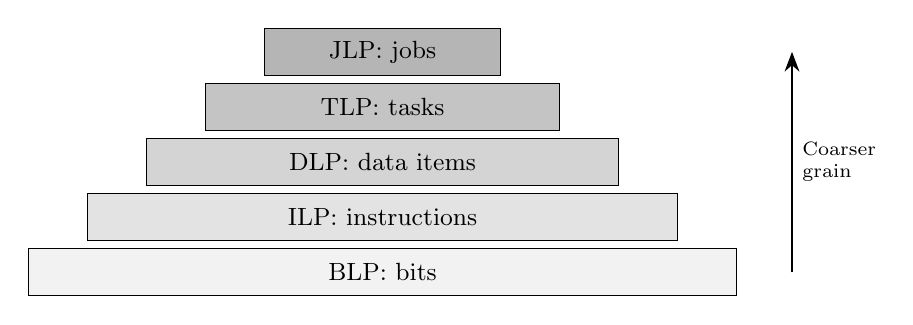
\begin{tikzpicture}
\foreach \i/\lab/\w in {0/BLP: bits/9,1/ILP: instructions/7.5,2/DLP: data items/6,3/TLP: tasks/4.5,4/JLP: jobs/3} {
\node[draw,minimum width=\w cm,minimum height=0.6cm,fill=black!\the\numexpr 5+\i*6\relax,font=\small] at (0,\i*0.7) {\lab};}
\draw[arr] (5.2,0)--(5.2,2.8) node[midway,right,font=\scriptsize,align=left]{Coarser\\grain};
\end{tikzpicture}
\figcap{Figure 18: Granularity of parallelism --- coarse-grain parallelism is built on top of fine-grain parallelism}
\end{center}

\textbf{Conclusion:} A modern processor explores all these types of parallelism. BLP, ILP, and DLP are well supported by advances in hardware and compilers. It is fair to say that \textbf{coarse-grain parallelism is built on top of fine-grain parallelism}.

%=========================================================
\section{Innovative Applications}
%=========================================================

\question{8}{Explain the innovative applications of HPC and HTC systems. What are their common requirements?}

Both HPC and HTC systems desire \textbf{transparency} in many application aspects. The following should be made transparent (hidden) from both users and system management:

\begin{center}
\renewcommand{\arraystretch}{1.25}
\small
\begin{tabularx}{0.9\linewidth}{|l|X|}
\hline
\textbf{Type of Transparency} & \textbf{The user does not need to know\ldots} \\ \hline
Data access & where or how the data is stored \\ \hline
Resource allocation & which machines are given to the job \\ \hline
Process location & on which computer the program is running \\ \hline
Concurrency in execution & that many other users are running jobs at the same time \\ \hline
Job replication & that copies of the job are running for safety \\ \hline
Failure recovery & that a machine failed and the system recovered \\ \hline
\end{tabularx}
\end{center}

\textbf{Applications of HPC and HTC systems (Table 1.1 of the textbook):}

\begin{center}
\renewcommand{\arraystretch}{1.25}
\small
\begin{tabular}{|p{4cm}|p{11cm}|}
\hline
\textbf{Domain} & \textbf{Specific Applications} \\ \hline
Science and engineering & Scientific simulations, genomic analysis; earthquake prediction, global warming, weather forecasting \\ \hline
Business, education, services industry, and health care & Telecommunication, content delivery, e-commerce; banking, stock exchanges, transaction processing; air traffic control, electric power grids, distance education; health care, hospital automation, telemedicine \\ \hline
Internet and web services, and government & Internet search, data centers, decision-making systems; traffic monitoring, worm containment, cyber security; digital government, online tax return processing, social networking \\ \hline
Mission-critical applications & Military command and control, intelligent systems, crisis management \\ \hline
\end{tabular}
\end{center}

\textbf{Common requirements:}
\begin{enumerate}
\item Almost all applications demand \textbf{computing economics}, \textbf{web-scale data collection}, \textbf{system reliability}, and \textbf{scalable performance}.
\item \textbf{Distributed transaction processing} is often practised in the banking and finance industry. Transactions represent \textbf{90 percent} of the existing market for reliable banking systems.
\item Users must deal with \textbf{multiple database servers} in distributed transactions.
\item Maintaining the \textbf{consistency of replicated transaction records} is crucial in real-time banking services.
\item Other complications include \textbf{lack of software support}, \textbf{network saturation}, and \textbf{security threats}.
\end{enumerate}

\begin{center}
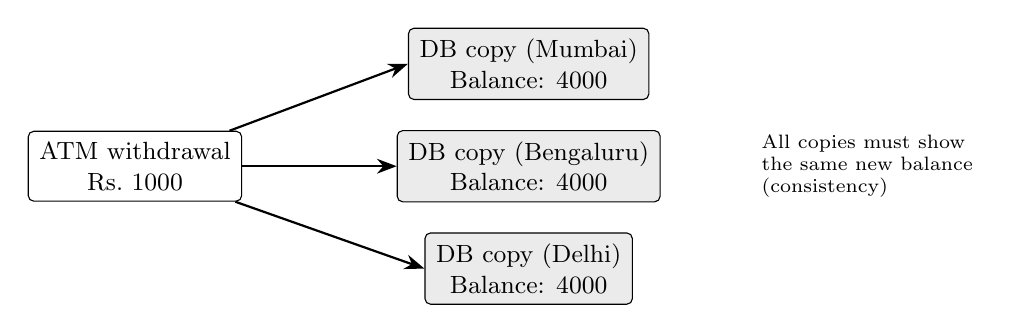
\begin{tikzpicture}
\node[box] (u) at (0,0) {ATM withdrawal\\Rs.\ 1000};
\foreach \i/\c in {0/Mumbai,1/Bengaluru,2/Delhi} \node[box,fill=black!8] (db\i) at (5,1.3-\i*1.3) {DB copy (\c)\\Balance: 4000};
\foreach \i in {0,1,2} \draw[arr] (u)--(db\i.west);
\node[font=\scriptsize,align=left] at (9.3,0) {All copies must show\\the same new balance\\(consistency)};
\end{tikzpicture}
\figcap{Figure 19: Consistency of replicated transaction records in banking}
\end{center}

%=========================================================
\section{The Trend toward Utility Computing}
%=========================================================

\question{8}{With a neat diagram, explain the vision of computer utilities in modern distributed computing systems. What is utility computing?}

\begin{center}
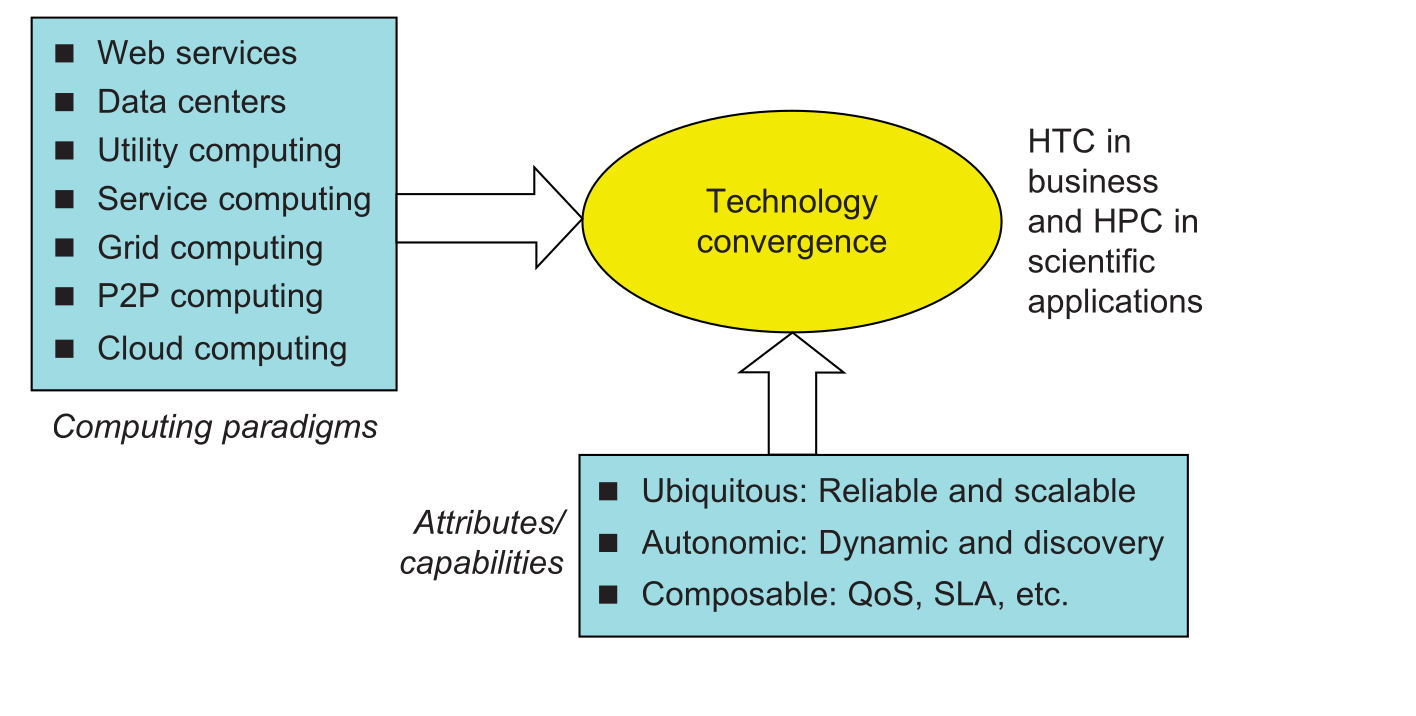
\includegraphics[width=0.66\linewidth]{images/Fig1_2_computer_utilities.png}
\figcap{Figure 20: The vision of computer utilities in modern distributed computing systems (Text Book 1, Fig.\ 1.2)}
\end{center}

\textbf{Explanation of the figure:}
\begin{enumerate}
\item \textbf{Computing paradigms (left box):} Web services, data centers, utility computing, service computing, grid computing, P2P computing, and cloud computing are the major paradigms used to study distributed systems.
\item \textbf{Attributes / capabilities (bottom box):} These paradigms share three common characteristics:
  \begin{itemize}
  \item \textbf{Ubiquitous:} They are present everywhere in daily life. \textbf{Reliability} and \textbf{scalability} are the two major design objectives.
  \item \textbf{Autonomic:} They aim at autonomic operations that can be \textbf{self-organized} to support \textbf{dynamic discovery}.
  \item \textbf{Composable:} They are composable with \textbf{QoS} (Quality of Service) and \textbf{SLAs} (Service-Level Agreements).
  \end{itemize}
\item \textbf{Technology convergence (centre):} The paradigms and their attributes converge together.
\item \textbf{Result (right):} This convergence supports \textbf{HTC in business} and \textbf{HPC in scientific applications}, and realizes the \textbf{computer utility vision}.
\end{enumerate}

\begin{defbox}
\textbf{Utility computing} focuses on a business model in which customers receive computing resources from a \textbf{paid service provider}, and pay according to usage, just like electricity or water.
\end{defbox}

\begin{center}
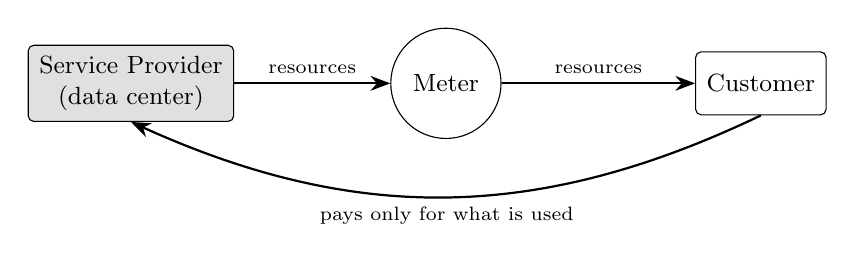
\begin{tikzpicture}
\node[box,fill=black!12] (p) at (0,0) {Service Provider\\(data center)};
\node[draw,circle,font=\small,minimum size=1.4cm] (m) at (4,0) {Meter};
\node[box] (c) at (8,0) {Customer};
\draw[arr] (p)--node[above,font=\scriptsize]{resources} (m);
\draw[arr] (m)--node[above,font=\scriptsize]{resources} (c);
\draw[arr] (c.south) to[bend left=25] node[below,font=\scriptsize]{pays only for what is used} (p.south);
\end{tikzpicture}
\figcap{Figure 21: Utility computing --- pay-per-use model}
\end{center}

\textbf{Points on utility computing:}
\begin{enumerate}
\item All grid and cloud platforms are regarded as \textbf{utility service providers}.
\item Cloud computing offers a \textbf{broader concept} than utility computing.
\item Distributed cloud applications run on any available servers in some \textbf{edge networks}.
\item \textbf{Technological challenges} include all aspects of computer science and engineering. Users demand:
  \begin{itemize}
  \item new network-efficient processors,
  \item scalable memory and storage schemes,
  \item distributed OSes,
  \item middleware for machine virtualization,
  \item new programming models,
  \item effective resource management, and
  \item application program development.
  \end{itemize}
\item These hardware and software supports are necessary to build distributed systems that explore \textbf{massive parallelism at all processing levels}.
\end{enumerate}

\textbf{Analogy:} We pay the electricity bill for the units consumed; we do not build a power plant at home.

%=========================================================
\section{The Hype Cycle of New Technologies}
%=========================================================

\question{8}{What is a hype cycle? With a neat diagram, explain the five stages of the hype cycle of new technologies.}

\begin{defbox}
A \textbf{hype cycle} is a graphical representation (by the research firm Gartner) of the expectations for an emerging technology at \textbf{five different stages}, from its introduction until its mainstream adoption.
\end{defbox}

\begin{center}
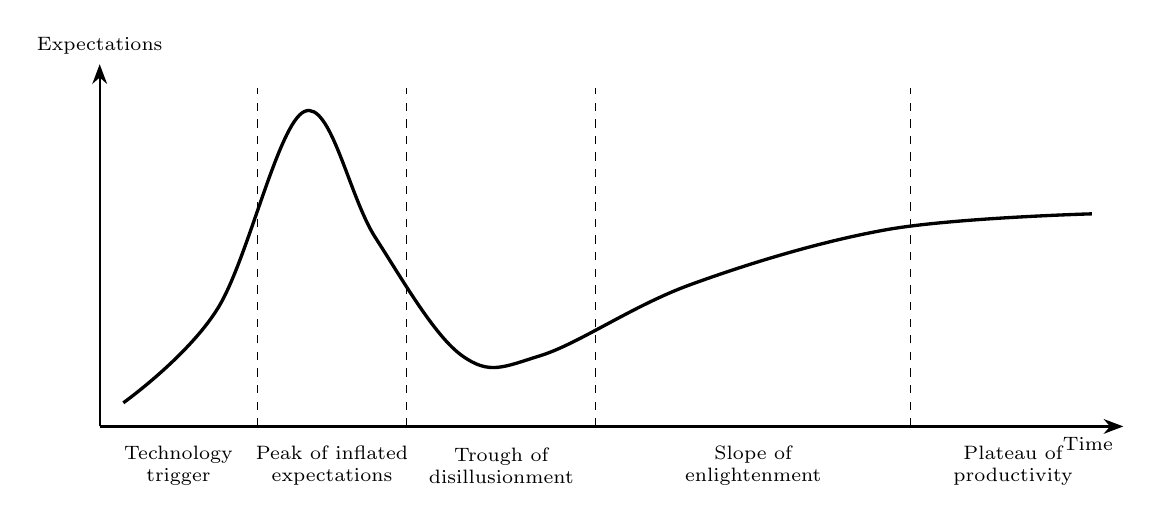
\begin{tikzpicture}[x=1cm,y=1cm]
\draw[arr] (0,0)--(13,0) node[below left,font=\scriptsize]{Time};
\draw[arr] (0,0)--(0,4.6) node[above,font=\scriptsize]{Expectations};
\draw[very thick] plot[smooth,tension=0.6] coordinates {(0.3,0.3) (1.5,1.5) (2.6,4.0) (3.5,2.4) (4.6,0.9) (5.6,0.9) (7.5,1.8) (10,2.5) (12.6,2.7)};
\foreach \x in {2,3.9,6.3,10.3} \draw[dashed] (\x,0)--(\x,4.3);
\node[font=\scriptsize,align=center] at (1,-0.5) {Technology\\trigger};
\node[font=\scriptsize,align=center] at (2.95,-0.5) {Peak of inflated\\expectations};
\node[font=\scriptsize,align=center] at (5.1,-0.5) {Trough of\\disillusionment};
\node[font=\scriptsize,align=center] at (8.3,-0.5) {Slope of\\enlightenment};
\node[font=\scriptsize,align=center] at (11.6,-0.5) {Plateau of\\productivity};
\end{tikzpicture}
\figcap{Figure 22: The five stages of the hype cycle}
\end{center}

\textbf{Five stages:}
\begin{enumerate}
\item \textbf{Technology trigger:} A new technology is introduced and expectations begin to rise.
\item \textbf{Peak of inflated expectations:} Expectations rise sharply from the trigger period to a high peak, often beyond what the technology can deliver.
\item \textbf{Trough of disillusionment:} Through a short period of disillusionment, expectations drop to a valley.
\item \textbf{Slope of enlightenment:} Expectations then increase steadily over a long enlightenment period as the real uses are understood.
\item \textbf{Plateau of productivity:} The technology reaches mainstream adoption and is productively used.
\end{enumerate}

Once a technology begins to climb the slope of enlightenment, it may reach the productivity plateau within \textbf{two to five years}.

\textbf{Hype cycle for emerging technologies, 2010:}

\begin{center}
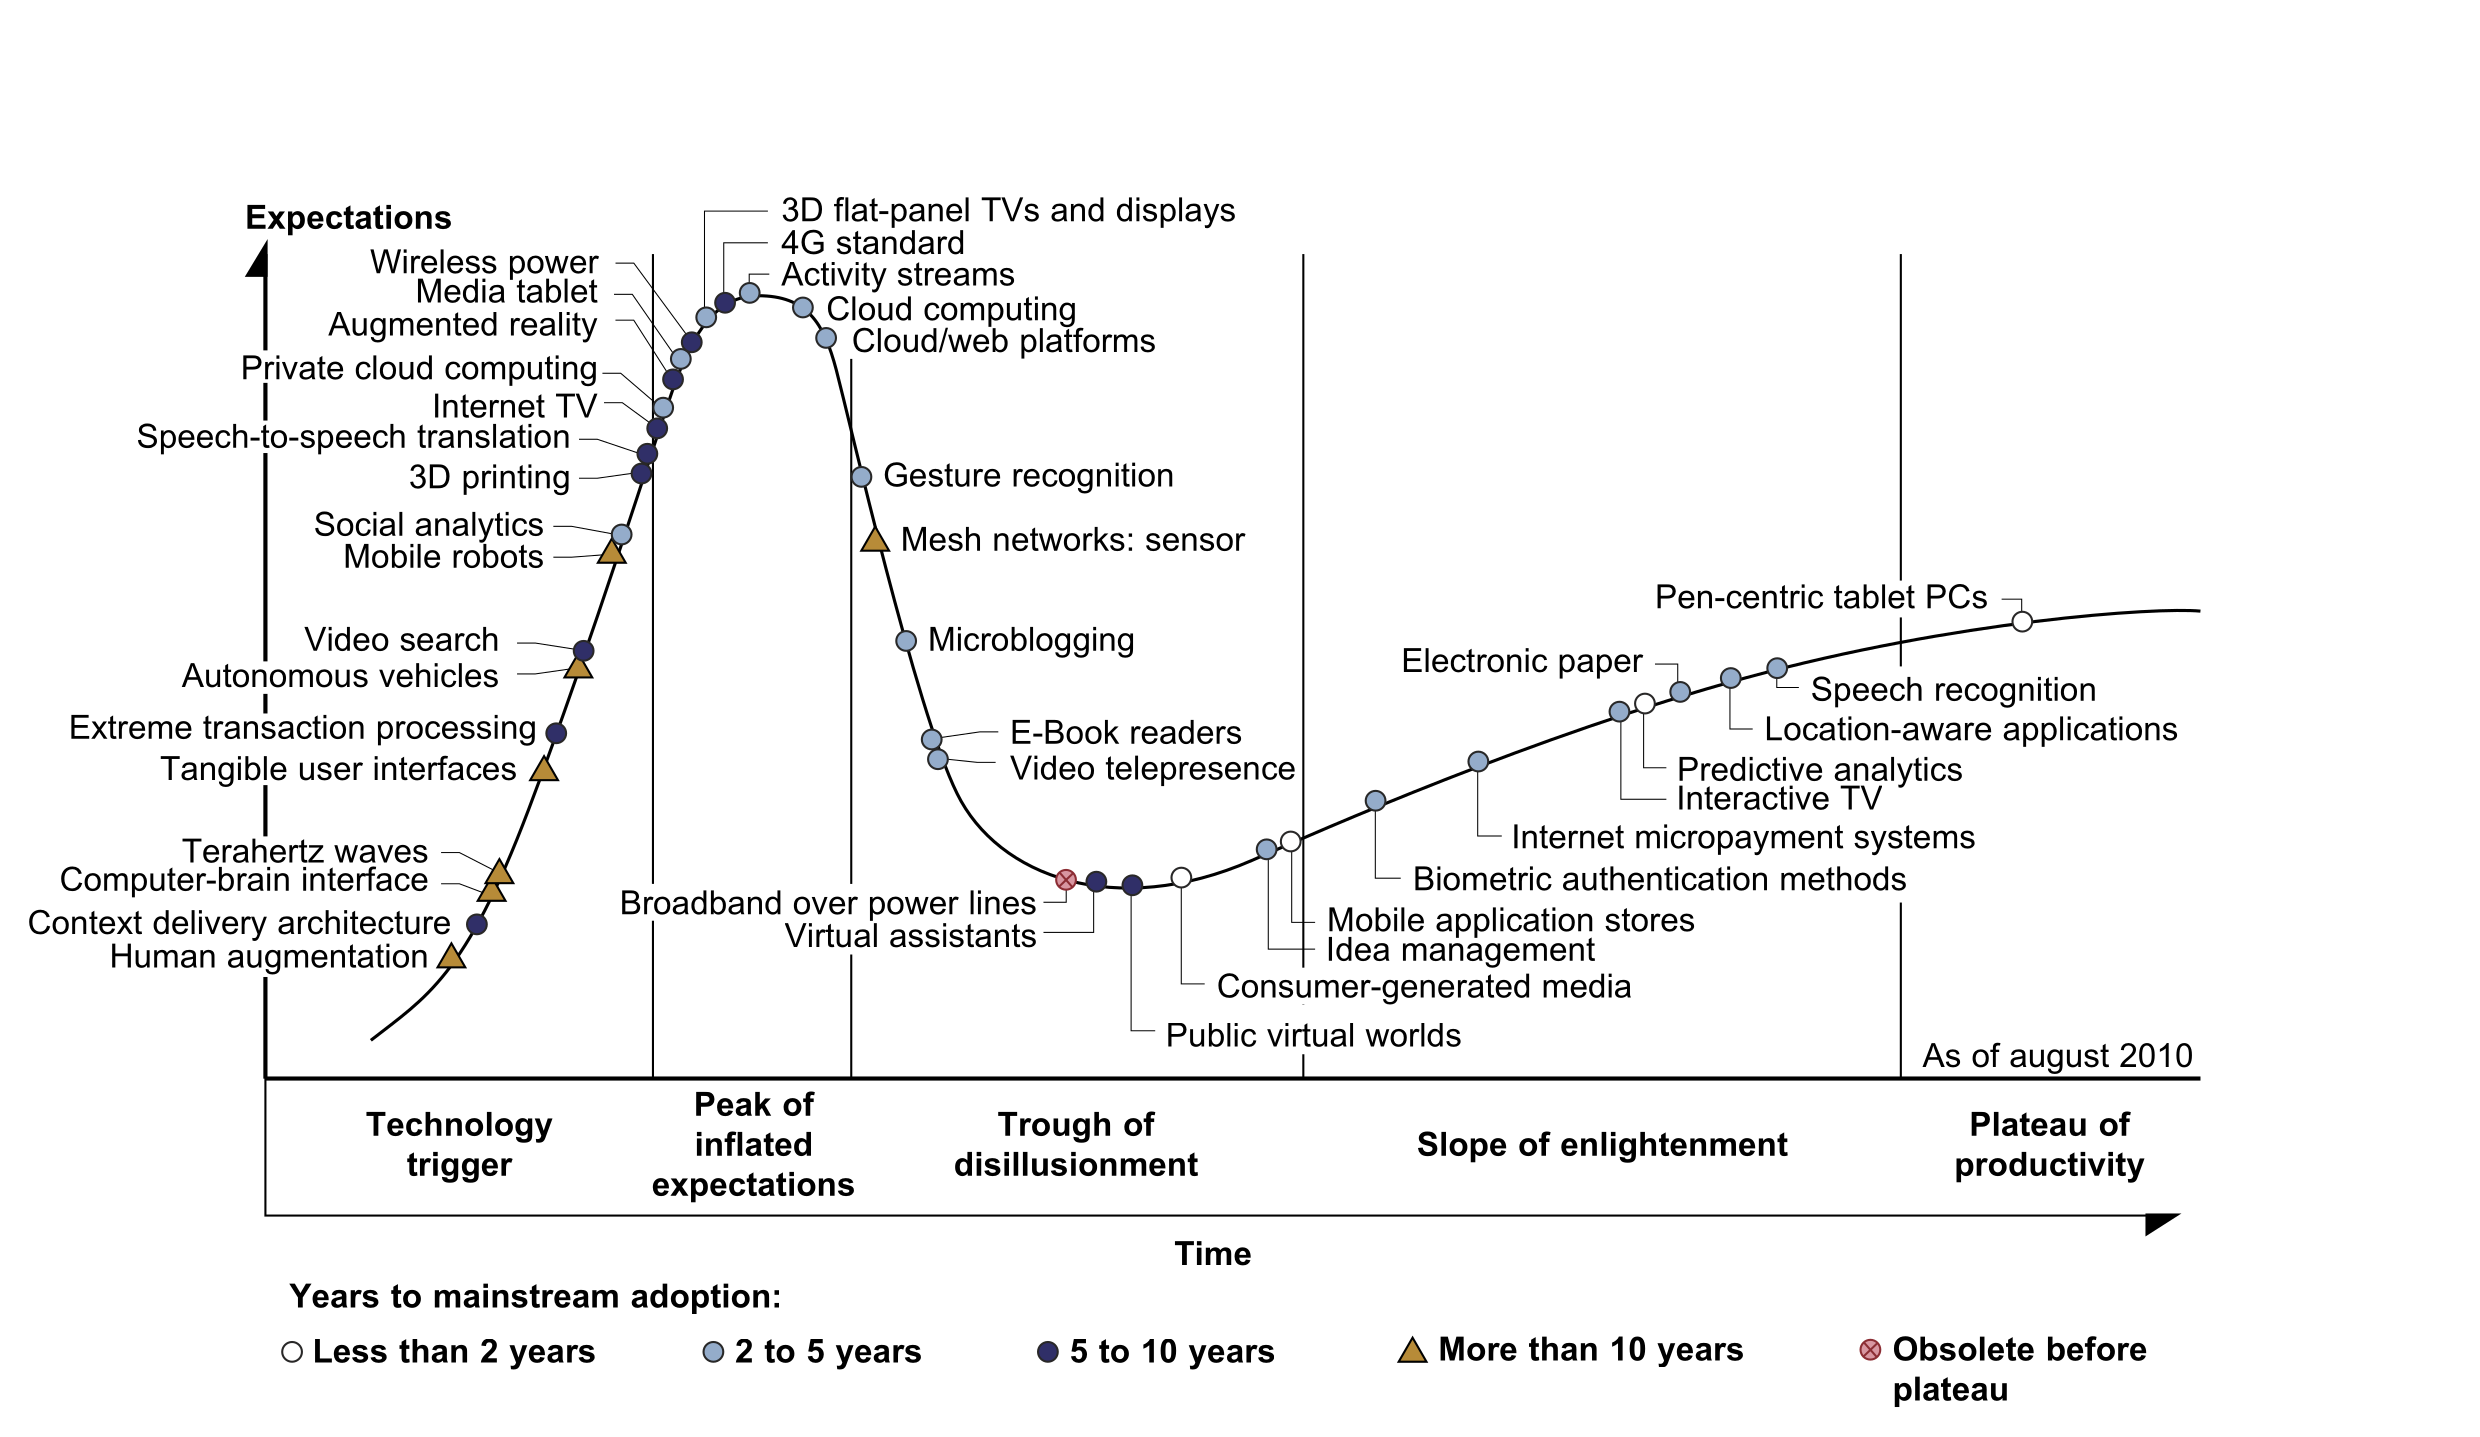
\includegraphics[width=0.9\linewidth]{images/Fig1_3_hype_cycle.png}
\figcap{Figure 23: Hype cycle for emerging technologies, 2010 (Text Book 1, Fig.\ 1.3; source: Gartner, Inc., 2010)}
\end{center}

\textbf{Symbols used (years to mainstream adoption):}
\begin{center}
\renewcommand{\arraystretch}{1.25}
\small
\begin{tabular}{|p{3.2cm}|p{3.6cm}|p{7.4cm}|}
\hline
\textbf{Symbol} & \textbf{Years to Mainstream} & \textbf{Example (as of August 2010)} \\ \hline
Hollow circle & Less than 2 years & Consumer-generated media (in the trough of disillusionment) \\ \hline
Gray circle & 2 to 5 years & Internet micropayment systems (enlightenment to maturity); cloud computing \\ \hline
Solid circle & 5 to 10 years & 3D printing (rising expectation stage) \\ \hline
Triangle & More than 10 years & Mesh network sensors (inflated expectation stage) \\ \hline
Crossed circle & Obsolete before plateau & Broadband over power lines \\ \hline
\end{tabular}
\end{center}

\textbf{Observations from the 2010 hype cycle:}
\begin{itemize}
\item \textbf{Cloud technology} had just crossed the peak of expectations in 2010 and was expected to take \textbf{two to five years} to reach the productivity stage.
\item \textbf{Broadband over power lines} was expected to become obsolete before leaving the trough of disillusionment.
\item Many technologies (dark circles) were at their peak in August 2010 and were expected to take five to ten years to reach the plateau.
\item Promising technologies included clouds, biometric authentication, interactive TV, speech recognition, predictive analytics, and media tablets.
\end{itemize}

%=========================================================
\section{Question Bank}
\label{sec:qbank}
%=========================================================

\begin{center}
\renewcommand{\arraystretch}{1.3}
\small
\begin{tabularx}{\linewidth}{|c|X|c|c|}
\hline
\textbf{Sl.} & \textbf{Question} & \textbf{Marks} & \textbf{Section} \\ \hline
1 & What is scalable computing over the Internet? Explain how computing has changed from centralized to parallel and distributed computing. & 6 & 1 \\ \hline
2 & Explain the age of Internet computing. Why is the Linpack benchmark no longer optimal? & 6 & 2 \\ \hline
3 & Explain the platform evolution of computer technology through five generations with examples. & 6 & 3 \\ \hline
4 & With a neat diagram, explain the evolutionary trend toward parallel, distributed, and cloud computing. & 8 & 4 \\ \hline
5 & What is HPC? Explain its characteristics. & 6 & 5.1 \\ \hline
6 & What is HTC? Why is market-oriented computing shifting from HPC to HTC? & 6 & 5.2 \\ \hline
7 & Differentiate between HPC and HTC with a neat diagram and examples. & 8 & 5.3 \\ \hline
8 & Explain the three new computing paradigms. How has the meaning of ``computer'' changed? & 8 & 6 \\ \hline
9 & Distinguish between centralized, parallel, distributed, and cloud computing with neat diagrams. & 8 & 7 \\ \hline
10 & Write short notes on concurrent computing, ubiquitous computing, IoT, and Internet computing. & 6 & 7.1 \\ \hline
11 & Explain distributed system families and the design objectives of future HPC and HTC systems. & 8 & 8 \\ \hline
12 & Explain scalable computing trends. State Moore's law and Gilder's law. & 6 & 9 \\ \hline
13 & Explain the different degrees of parallelism with neat diagrams. & 8 & 10 \\ \hline
14 & Explain the innovative applications of HPC and HTC systems and their common requirements. & 8 & 11 \\ \hline
15 & With a neat diagram, explain the vision of computer utilities. What is utility computing? & 8 & 12 \\ \hline
16 & What is a hype cycle? Explain its five stages with a neat diagram. & 8 & 13 \\ \hline
17 & What is transparency in distributed systems? List the aspects that must be made transparent. & 6 & 11 \\ \hline
18 & Explain the design objectives: efficiency, dependability, adaptation, and flexibility. & 6 & 8 \\ \hline
\end{tabularx}
\end{center}

\end{document}